\documentclass[11pt]{article}
\usepackage{amsmath,amssymb,amsthm}
\usepackage[margin=1.05in]{geometry}
\usepackage{booktabs}
\usepackage{array}
\usepackage{graphicx}
\usepackage{microtype}
\usepackage[colorlinks=true,linkcolor=blue,citecolor=blue,urlcolor=blue]{hyperref}
\usepackage{xurl}
\hypersetup{pdftitle={Certified ceilings for a Mertens-type extremal linear
  program},pdfauthor={Kevin Russell (ProjectForty2 / CHRONOS agent)}}

\newtheorem{theorem}{Theorem}
\newtheorem{lemma}[theorem]{Lemma}
\newtheorem{proposition}[theorem]{Proposition}
\newtheorem{corollary}[theorem]{Corollary}
\theoremstyle{remark}
\newtheorem{remark}[theorem]{Remark}

\newcommand{\NN}{\mathbb{N}}
\newcommand{\RR}{\mathbb{R}}
\newcommand{\ZZ}{\mathbb{Z}}
\newcommand{\Sstar}{S^{*}}
\DeclareMathOperator{\supp}{supp}

\title{Certified ceilings for a Mertens-type extremal linear program,\\
with exact dual certificates at reaches $4800$ and $12000$}
\author{Kevin Russell\thanks{%
Correspondence: \texttt{kevinrussell@gmail.com}. Computer-assisted note,
prepared with CHRONOS, ProjectForty2's autonomous research agent; the author
takes responsibility for all claims. The \emph{constructions} and
leaderboard measurements discussed in Section~\ref{sec:measure} are due to
the agents ``Agent-Knowledge-Cycle'' and ``JSAgent'' on the EinsteinArena
platform \cite{AKC26,JSAgent26}; see the attribution statement in
Section~\ref{sec:intro}. Verification artifacts are listed in
Appendix~\ref{sec:repro}.}\\[3pt]
{\normalsize ProjectForty2 --- CHRONOS agent}}
\date{July 6, 2026}

\begin{document}
\maketitle

\begin{abstract}
For $K \in \NN$ and tolerance $\tau = 1.0001$, let
\begin{multline*}
\Sstar(K) \;=\; \max\Bigl\{\, -\sum_{k=2}^{K} f(k)\,\frac{\ln k}{k}
\;:\; f \in [-10,10]^{K-1},\\
\sum_{k=2}^{K} f(k)\Bigl(\Bigl\lfloor\frac{m}{k}\Bigr\rfloor -
\frac{m}{k}\Bigr) \le \tau \text{ for } m = 1, \dots, 10K-1 \Bigr\},
\end{multline*}
the extremal value of the scoring rule of the EinsteinArena
``prime-number-theorem'' benchmark board. We prove
\[
\Sstar(4800) \;\le\; 0.9963688817172828744325041,
\quad
\Sstar(12000) \;\le\; 0.9974876103072528157057480,
\]
by weak-duality \emph{box certificates}: explicit dyadic-rational dual
vectors $y = Y/2^{48}$, entrywise nonnegative, whose certified bound
$B(y) = \tau \sum_m y_m + 10 \sum_k |r_k|$ is evaluated with exact integer
residual accumulation and outward-rounded $400$-bit interval enclosures of
$\ln k / k$; no unenclosed floating-point scalar enters the certified
inequality --- every transcendental quantity is replaced by an
outward-rounded high-precision interval, and the log enclosures are
themselves cross-audited (dual-precision nesting at $400$ vs $800$ bits over
every $k$, plus a rational $\operatorname{atanh}$-series bracket independent
of any log oracle) --- and an independent skeptic harness (fresh residual
computation by a different route, pure-rational spot checks, hash pinning)
passes all checks on both certificates. Numerically, the certificates are close to the
floating-point LP optima, which sit $5.6\times10^{-7}$ (reach $4800$) and
$2.7\times10^{-5}$ (reach $12000$) below the certified ceilings (these
optima are float measurements, not a certified lower bracket). The problem is a finite Mertens-type program:
the M\"obius function is its infinite-reach extremal shadow --- $\mu$
satisfies the constraint with $E(m) \equiv 1$ and objective $1$, both
classical equivalents of the prime number theorem --- but no finite
truncation of $\mu$ is feasible (measured violation $104.2$ at reach
$48000$), which is why the board's leaders are sparse feasible surrogates
rather than truncated M\"obius. Alongside the two theorems we report
measurements (floats, clearly labeled, none of them certificates): the
reach-$12000$ optimal support is dense ($10255$ of $11999$ keys), a
cardinality-penalty curve quantifying the board's $2000$-key cap, and a
certified bracket for the structure-constant question raised by the
competition agents --- the certified floor $c^*(4800) \approx 0.0391$ shows
their family's plateau constant $c \approx 0.036$ is unattainable at reach
$4800$, while at reach $12000$ the floor drops to $0.02938$ and the best
measured $2000$-key support reaches only $c \approx 0.0413$, so the capped
question stays open in both directions. Items not machine-verified at the
time of writing, including the still-running reach-$24000$ certificate, are
listed in a pending-verification ledger.
% PREPRINT-ONLY LINE: the closing sentence below is kept for the preprint;
% trim it for a journal version (per referee minor (d)).
A ceiling is not a construction:
nothing on the leaderboard moves because of this note.
\end{abstract}

\medskip
\noindent\textbf{MSC 2020:} 90C05 (primary); 11N37, 90C57, 65G30
(secondary).\\
\textbf{Keywords:} linear programming duality; computer-assisted proof;
exact rational arithmetic; M\"obius function; certification of numerical
records.

\section{Introduction}\label{sec:intro}

This note certifies \emph{ceilings} --- rigorous upper bounds on the best
possible value --- for a family of finite linear programs whose origin is a
live optimization benchmark. On the EinsteinArena platform, the board
\texttt{prime-number-theorem} asks agents to submit a partial function
$f\colon \{2,\dots\} \to [-10,10]$ (at most $2000$ keys) and scores it by
$-\sum_k f(k) \ln k / k$, subject to a verifier constraint recalled in
Section~\ref{sec:program}; the top of the leaderboard has moved
$0.99632 \to 0.99652 \to 0.99715 \to 0.99735 \to 0.99740$ over recent weeks
as agents push the \emph{reach} (the largest key used) from $16000$ to
$63998$. All leaderboard values are floating-point scores of explicit
constructions; none of them, and no value previously discussed on the
board, came with a proof of how high the score \emph{can} go at a given
reach. The two theorems below supply exactly that missing object at reaches
$4800$ and $12000$: certified, exact-arithmetic upper bounds on the full
program value $\Sstar(K)$, valid for every legal submission at those
reaches, sitting $5.6\times10^{-7}$ and $2.7\times10^{-5}$ above the
respective LP optima.

\paragraph{Why ``prime-number-theorem''.} The program is a finite,
box-constrained relative of Mertens-type sums. As Section~\ref{sec:mobius}
recalls, the M\"obius function satisfies the constraint \emph{exactly}
($E(m) \equiv 1$ for every $m$, by an elementary identity), and its
objective value is $1$ --- the statements $\sum_k \mu(k)/k = 0$ and
$-\sum_k \mu(k) \ln k / k = 1$ being classical equivalents of the prime
number theorem. So the board's score has a natural asymptote at the
tolerance $\tau$, approached by $\tau\mu$; but no finite truncation of
$\mu$ is feasible (we measure a constraint violation of $104.2$ at reach
$48000$), and the interesting mathematics of the competition is which
\emph{sparse feasible surrogates} for $\mu$ score best under a $2000$-key
budget.

\paragraph{What this note proves.} Theorems~\ref{thm:k4800}
and~\ref{thm:k12000} are weak-duality certificates in the sense of
Proposition~\ref{prop:box}: explicit nonnegative dyadic-rational dual
vectors $y = Y/2^{48}$ whose certified bound
$B(y) = \tau\sum_m y_m + 10 \sum_k |r_k|$ dominates $\Sstar(K)$. The
certified path is exact end to end --- integer residual accumulation via
$\sum_m Y_m\,(m \bmod k)$, outward-rounded interval enclosures of
$\ln k/k$ at $400$ bits, directed decimal round-up --- and each certificate
was re-verified by an independent skeptic harness
(Section~\ref{sec:method}). Everything else in the note --- the support
density, the cardinality-penalty curve, the structure-constant bracket of
Section~\ref{sec:measure} --- is measurement: floating-point values of
explicit solves, clearly labeled, confirmed against the platform's own
verifier where a legal submission exists, and never called a theorem.

\paragraph{Attribution.} This is a certification exercise on a live
competition, and credit belongs where the mathematics originated. The
multiscale support family driving the current leaderboard (a dense
squarefree prefix up to $1800$ plus a geometric squarefree tail), the
gap decomposition $1 - S \approx c/\ln(10\cdot\mathrm{reach})$, and an
honest reach ladder for it were published on the board by the agent
``Agent-Knowledge-Cycle'' \cite{AKC26}; the reach-$48000$ and
reach-$64000$ extensions that hold the lead, the measurement that the
family's structure constant has plateaued at $c \approx 0.0360$--$0.0361$,
and the question of whether \emph{any} $2000$-key family goes below
$0.036$ are due to the agent ``JSAgent'' \cite{JSAgent26}. Our contribution
is the two certified ceilings, the certificate and skeptic machinery, and
the measurements of Section~\ref{sec:measure}; the certificate method
continues the exact-arithmetic program of our earlier notes on the
Erd\H{o}s minimum overlap constant \cite{ErdosNote26} and on
autoconvolution inequalities \cite{AutocorrNote26}. This note itself was
drafted and verified computer-assisted, by CHRONOS, ProjectForty2's
autonomous research agent, operating under the author's direction; the
author reviewed the mathematics and takes full responsibility for all
claims.

\section{The program and the deployed verifier}\label{sec:program}

Fix the tolerance $\tau = 1.0001$ and a reach $K \in \NN$. For
$f = (f(2), \dots, f(K)) \in [-10,10]^{K-1}$ define
\begin{equation}\label{eq:E}
E_f(m) \;=\; \sum_{k=2}^{K} f(k) \Bigl( \Bigl\lfloor \frac{m}{k}
\Bigr\rfloor - \frac{m}{k} \Bigr), \qquad m \in \NN,
\end{equation}
and the program
\begin{equation}\label{eq:prog}
\Sstar(K) \;=\; \max \Bigl\{ -\sum_{k=2}^{K} f(k)\, \frac{\ln k}{k}
\;:\; E_f(m) \le \tau \text{ for all } m \in \{1, \dots, 10K - 1\},\;
f \in [-10,10]^{K-1} \Bigr\} .
\end{equation}
The feasible set is a nonempty compact polytope ($f \equiv 0$ is
feasible), so the maximum exists.

\subsection{Provenance: reduction of the board semantics}
\label{sec:verifier}

Program~\eqref{eq:prog} is the exhaustive version of the deployed scoring
rule. The platform's verifier, whose source is public, does the following
with a submitted dictionary $\{k \mapsto v_k\}$: it rejects more than
$2000$ keys, clips each value to $[-10,10]$, sets
\begin{equation}\label{eq:f1}
f(1) \;=\; -\sum_{k} \frac{f(k)}{k}
\end{equation}
(so that $\sum_{k\ge1} f(k)/k = 0$), draws $10^7$ samples
$x \sim \mathrm{Uniform}[1, 10K_s)$ with a \emph{fixed} pseudorandom seed,
where $K_s$ is the largest submitted key, rejects the submission if
$\sum_k f(k) \lfloor x/k \rfloor > \tau$ at any sample, and otherwise
returns the score $-\sum_k f(k) \ln k / k$ (the synthesized $k=1$ term
contributes $0$ to the score since $\ln 1 = 0$).

\begin{lemma}[the sampled verifier evaluates integer constraints;
sampling scope]\label{lem:verifier}
Set $s = \sum_{k=2}^{K} f(k)/k$, so that the verifier's adjustment
\eqref{eq:f1} reads $f(1) = -s$, and let the verifier's raw constraint
functional be
\[
V(x) \;=\; f(1)\lfloor x\rfloor \;+\; \sum_{k=2}^{K} f(k)
\Bigl\lfloor \frac{x}{k} \Bigr\rfloor , \qquad x \ge 1 .
\]
\begin{enumerate}
\item[(i)] For every real $x \ge 1$, $V(x) = E_f(\lfloor x \rfloor)$, where
$E_f$ is the drift-free integer functional \eqref{eq:E}. In particular a
verifier sample drawn at any $x$ with $\lfloor x \rfloor = m$ tests
\emph{exactly} the integer constraint $E_f(m) \le \tau$.
\item[(ii)] Hence the constraint set enforced by any sample set
$X \subset [1, 10K_s)$ is $\{ E_f(m) \le \tau : m \in \lfloor X \rfloor
\}$, a subset of the constraints of \eqref{eq:prog} when $K_s = K$; the
exhaustive version is \eqref{eq:prog} itself.
\item[(iii)] The key cap and the value clipping only shrink the feasible
set of \eqref{eq:prog}.
\end{enumerate}
\end{lemma}

\begin{proof}
(i) Fix $x \in [1,\infty)$ and set $m = \lfloor x \rfloor$. For each
integer $k \ge 1$ the map $t \mapsto \lfloor t/k \rfloor$ is constant on
$[m, m+1)$: it jumps only at integer multiples of $k$, and the only integer
in $[m, m+1)$ is $m$ itself, so $\lfloor x/k \rfloor = \lfloor m/k \rfloor$
for every $k \ge 1$ (in particular $\lfloor x \rfloor = \lfloor x/1 \rfloor
= m$). Therefore
\[
V(x) \;=\; f(1)\,m + \sum_{k=2}^{K} f(k)\Bigl\lfloor \frac{m}{k}\Bigr\rfloor
\;=\; -s\,m + \sum_{k=2}^{K} f(k)\Bigl\lfloor \frac{m}{k}\Bigr\rfloor ,
\]
using $f(1) = -s$. Now substitute $s = \sum_{k=2}^{K} f(k)/k$ and regroup:
\[
V(x) \;=\; \sum_{k=2}^{K} f(k)\Bigl(\Bigl\lfloor \frac{m}{k}\Bigr\rfloor
- \frac{m}{k}\Bigr) \;=\; E_f(m) \;=\; E_f(\lfloor x \rfloor) .
\]
This is an exact identity between the verifier's raw floor sum $V(x)$ and
the drift-free integer functional $E_f$ evaluated at $\lfloor x \rfloor$;
no cancellation is asserted about the individual real drift terms $x/k$,
only that they reassemble into $E_f(m)$ once $f(1) = -s$ is used. (ii) By
(i), a sample at $x$ imposes $E_f(\lfloor x\rfloor) \le \tau$, an integer
constraint of \eqref{eq:prog}; ranging over $X$ gives the stated subset.
(iii) Fewer allowed keys and a smaller box are subsets.
\end{proof}

\begin{proposition}[realized coverage of the deployed sampler]
\label{prop:coverage}
Replicating the verifier's sampler bit-for-bit (same fixed seed, same
sequential draw of $10^7$ uniforms; the verifier's internal batching does
not affect the sample stream), the set
$\lfloor X \rfloor$ realizes \emph{every} integer $m \in \{1, \dots,
10K-1\}$ at all four reaches we checked: $0$ unmonitored intervals out of
$47\,999$ ($K = 4800$), $119\,999$ ($K = 12000$), $479\,999$
($K = 48000$), and $639\,999$ ($K = 64000$). The expected numbers of
unmonitored intervals are about $1.6\times10^{-86}$, $7.7\times10^{-32}$,
$4.3\times10^{-4}$, and $0.105$ respectively.
\end{proposition}

This is a computation, not a probabilistic claim: the seed is fixed, so
coverage is a deterministic property of the deployed code, and it is
complete at the reaches relevant to this note and to the current board.
Consequently, by Lemma~\ref{lem:verifier}, \emph{a submission with largest
key $K \in \{4800, 12000\}$ accepted by the deployed verifier is feasible
for \eqref{eq:prog}}, and every certified upper bound on $\Sstar(K)$
bounds its score. (For largest key $K' < K$ the verifier enforces the
reach-$K'$ program; see Remark~\ref{rem:monotone}.)

\section{The M\"obius shadow}\label{sec:mobius}

\begin{remark}[why the board bears the name]\label{rem:mobius}
Let $\mu$ be the M\"obius function. Three classical facts:
\begin{enumerate}
\item[(a)] $\sum_{k \le x} \mu(k) \lfloor x/k \rfloor = 1$ for every real
$x \ge 1$ \cite[Theorem 3.12]{Apostol76} (an identity, no PNT needed);
\item[(b)] $\sum_{k=1}^{\infty} \mu(k)/k = 0$;
\item[(c)] $-\sum_{k=1}^{\infty} \mu(k) \ln k / k = 1$;
\end{enumerate}
the convergence statements (b) and (c) are classically equivalent to the
prime number theorem \cite[Ch.~4]{Apostol76}. By (a) and (b), the full
M\"obius function --- as an ``infinite submission'' on keys $k \ge 2$,
values $\mu(k) \in \{-1,0,1\}$, with the $f(1)$-adjustment
\eqref{eq:f1} synthesizing $f(1) = 1 - 0 = \mu(1)$ in the limit --- has
$E_\mu(m) = 1$ \emph{identically}, hence is feasible for every $\tau \ge
1$, with objective $1$ by (c); and $\tau\mu$ is feasible with objective
$\tau$. The board's score therefore has asymptote $\tau = 1.0001$, and the
observed leader progression $0.99632 \to 0.99740$ is a march up this
asymptote.

No finite truncation participates in this, however. For
$\mu$ truncated at reach $K$ the identity (a) still forces
$E(m) = 1 - m T_K$ for $m \le K$, where $T_K = \sum_{k \le K} \mu(k)/k$
--- feasible when $T_K > 0$ --- but for $m \in (K, 10K)$ the cancellation
in (a) is cut and the constraint fails badly: we measured (floating point,
reported as measurement)
\begin{gather*}
\max_{m < 480000} E(m) = 104.212 \;\;\text{at } m = 285645
\quad (K = 48000),\\[1pt]
\max_{m < 640000} E(m) = 200.199 \quad (K = 64000),
\end{gather*}
both wildly above $\tau$. The competition's constructions are thus
genuinely different objects: sparse supports engineered to be feasible on
the \emph{whole} window $[1, 10K)$, for which $\mu$ is only the
infinite-reach shadow.
\end{remark}

\section{The certificate method}\label{sec:method}

\subsection{Weak-duality box certificates}

Write $c_k = -\ln k / k$ and $a_{m,k} = \lfloor m/k \rfloor - m/k$ for
$2 \le k \le K$ and $1 \le m \le 10K - 1$, so that \eqref{eq:prog} is
$\max \{ c^{\mathsf T} f : A f \le \tau \mathbf{1},\ \|f\|_\infty \le 10
\}$.

\begin{proposition}[box certificate]\label{prop:box}
Let $y = (y_m)_{m \in M_0} \ge 0$ be any finite nonnegative vector indexed
by a set $M_0 \subseteq \{1, \dots, 10K-1\}$, and define the residuals
\[
r_k \;=\; c_k - \sum_{m \in M_0} y_m\, a_{m,k}, \qquad 2 \le k \le K .
\]
Then
\[
\Sstar(K) \;\le\; B(y) \;:=\; \tau \sum_{m \in M_0} y_m \;+\;
10 \sum_{k=2}^{K} |r_k| .
\]
The same bound holds for any program whose constraint set contains
$\{ E_f(m) \le \tau : m \in M_0 \}$ --- in particular for the sampled
verifier whenever its realized coverage includes $M_0$.
\end{proposition}

\begin{proof}
For feasible $f$,
$c^{\mathsf T} f = \sum_k r_k f_k + \sum_{m} y_m \sum_k a_{m,k} f_k
\le 10 \sum_k |r_k| + \tau \sum_m y_m$, using $|f_k| \le 10$,
$y_m \ge 0$, and $E_f(m) \le \tau$ for $m \in M_0$. Only the constraints
in $M_0$ were used.
\end{proof}

\subsection{The exact path}\label{sec:exact}

A certificate is only as rigorous as its evaluation. Both certificates
below follow the same exact path:
\begin{enumerate}
\item \textbf{Dyadic dual.} The solver's dual vector is converted to
$y_m = Y_m / 2^{48}$ with integer $Y_m \ge 0$ (negative entries would be
clipped and counted; the count is $0$ for both certificates, and the
skeptic re-verifies $\min_m Y_m \ge 0$). The support sizes are $4800$
rows ($K = 4800$) and $12058$ rows ($K = 12000$), in both cases with
$\max m \le 10K - 1$, so Proposition~\ref{prop:box} applies with
$M_0 \subseteq \{1,\dots,10K-1\}$.
\item \textbf{Integer residuals.} Since $k\lfloor m/k\rfloor - m =
-(m \bmod k)$,
\[
r_k \;=\; -\frac{\ln k}{k} \;+\; \frac{1}{k\, 2^{48}}
\sum_{m} Y_m\, (m \bmod k),
\]
and the inner sum is a plain nonnegative big integer, accumulated exactly.
\item \textbf{Interval enclosures.} $\ln k / k$ is enclosed in
\texttt{mpmath} interval arithmetic at $400$ bits; every $|r_k|$ is
replaced by the upper end of its enclosure, every sum is outward-rounded,
and the final $B$ is rounded \emph{up} to $25$ decimal digits. No
unenclosed floating-point approximation enters the certified inequality:
the only non-exact quantities are the transcendentals $\ln k$, each of which
appears solely through an outward-rounded interval, so the accumulated bound
is a rigorous over-estimate of the exact $B(y)$.
\item \textbf{Skeptic.} An independent harness then (i) recomputes the
SHA-256 hash of the integer dual and checks it against the certificate,
(ii) re-checks scoping ($K$, $10K$, $\tau$, box, row range, nonnegativity),
(iii) recomputes $r_k$ at $20$ random $k$ by pure
\texttt{fractions.Fraction} arithmetic --- deliberately \emph{not} reusing
the certifier's $m \bmod k$ shortcut --- and compares against the claimed
$\max_k |r_k|$, (iv) runs a full independent residual pass and re-derives
$B$, checking it against the certified decimal, and (v) checks
$B \ge$ both floating primal values. Verdict on both certificates:
\textsc{all pass}.
\end{enumerate}

\subsection{Auditing the log enclosures}\label{sec:logaudit}

The single non-exact ingredient of the certified path is the family of
enclosures of $\ln k$ ($2 \le k \le K$), produced by \texttt{mpmath}'s
interval-log routine. To avoid resting the bound on that one oracle we
verified the enclosures two independent ways; both audits pass at $K=4800$
and $K=12000$, with machine-readable summaries archived
(Appendix~\ref{sec:repro}).

\textbf{(a) Dual-precision nesting, over every $k$.} For each $k = 2,\dots,K$
the enclosure of $\ln k / k$ was recomputed at $400$ and at $800$ bits, and
the exact rational endpoints of both intervals were extracted directly from
the interval mantissa/exponent representation (reading the raw endpoint
tuples, rather than casting through \texttt{mpmath}'s \texttt{mpf}, which
would silently re-round at the ambient working precision). The $800$-bit
interval was confirmed to nest inside the $400$-bit interval for every $k$:
$0$ nesting failures at both reaches. The widest $\ln k / k$ enclosure
(worst case $k=3$) has width $3.9\times10^{-121}$ at $400$ bits and
$1.5\times10^{-241}$ at $800$ bits, so the certifier's $400$-bit enclosures
are already orders of magnitude tighter than the $\sim10^{-25}$ granularity
of the final bound and agree with the $800$-bit refinement.

\textbf{(b) A rational bracket with no transcendental oracle.} As a
cross-check that the log routine is not merely self-consistent, we bracketed
$\ln k$ on a spread of $21$ keys, namely $k =$
2, 3, 5, 7, 10, 13, 17, 23, 31, 47, 64, 97, 128, 251, 320, 323, 389, 428,
429, 512, 730, by pure rational arithmetic via
$\ln k = 2\operatorname{atanh}\!\bigl(\tfrac{k-1}{k+1}\bigr)$: the partial
sum of the (all-positive) $\operatorname{atanh}$ power series is a rigorous
rational lower bound, and the geometric tail estimate
$u^{2N+1}/\bigl((2N+1)(1-u^{2})\bigr)$ with $u=\tfrac{k-1}{k+1}$ is a
rigorous rational upper bound, with the term count chosen adaptively to a
target width of $10^{-20}$ (achieved worst-case width $10^{-20}$). No
transcendental function is called anywhere in this bracket. Every
\texttt{mpmath} interval was confirmed consistent with (i.e.\ overlapping,
and jointly enclosing $\ln k$ with) the corresponding rational bracket:
$0$ disagreements at both reaches. The rational bracket is capped at
$k \le 1000$ because its running big-integer \texttt{Fraction} cost grows
with $k$; the $2$--$730$ spread is representative, and audit (a) already
covers every $k$ up to $K$ at full strength.

\subsection{Computation: making the LP solvable}\label{sec:compute}

The constraint matrix of \eqref{eq:prog} is dense: $a_{m,k} \ne 0$ for
essentially all $(m,k)$, giving $\approx 2.3\times10^{10}$ nonzeros at
$K = 48000$ --- unassemblable. Two standard devices make the family
tractable, recorded here because the second contains a documented negative
result that cost real time.

\textbf{Chain reformulation.} Introduce running values
$t_m = \sum_k f(k)\lfloor m/k \rfloor - m s$ with a drift variable
$s = \sum_k f(k)/k$. Then $t_m - t_{m-1} - \sum_{k \mid m} f(k) + s = 0$,
so the dense rows become sparse chain rows whose nonzero count is
$\sum_{m < 10K} d_{[2,K]}(m) + O(10K) \approx 10K \ln(10K)$: at
$K = 48000$ the assembled model has $6\,435\,399$ nonzeros instead of
$2.3\times10^{10}$ ($1\,442\,520$ at $K = 12000$).

\textbf{Constraint generation.} Only bound rows $t_m \le \tau$ near the
binding set are activated, by violation scans between rounds; the
reach-$12000$ solve converged in $12$ rounds with a working set of
$94\,181$ of $119\,999$ bound rows.

\textbf{Documented finding: cold dual simplex stalls in phase 1 on this
family.} The single-LP attempt at $K = 48000$ ran dual simplex for
$3\,858\,475$ iterations and was aborted at its $72\,000$-second
($20$-hour) time limit, still short of optimality --- no valid duals were
produced, and no certificate exists at that reach
(Section~\ref{sec:pending}). A cold dual-simplex round at $K = 24000$ was
still in simplex phase 1 after $4$ hours ($196\,092$ infeasibilities at
the last log line). By contrast, interior point with crossover solved the
round-1 relaxations easily (head-to-head at $K = 6000$: $60.2$\,s dual
simplex vs $11.9$\,s IPM), and a reach-$12000$ resolve round on which warm
dual simplex twice hit a $2700$-second limit completed under IPM in
$1381$\,s. The production configuration --- IPM$+$crossover in round 1,
IPM resolves --- is what produced both certified duals.

\section{The theorems}\label{sec:theorems}

\begin{theorem}[reach-$4800$ ceiling]\label{thm:k4800}
With $\Sstar$ as in \eqref{eq:prog} and $\tau = 1.0001$,
\[
\Sstar(4800) \;\le\; 0.9963688817172828744325041 .
\]
\end{theorem}

\begin{proof}
Apply Proposition~\ref{prop:box} with the explicit dual
$y = Y/2^{48}$, $Y \in \ZZ_{\ge0}^{4800}$ (row support
$\subseteq [1, 47982]$; dual SHA-256 beginning \texttt{b13f05d2}, given in
full in Appendix~\ref{sec:repro}), archived with the certificate. Its
exact mass is
\[
\sum_m y_m \;=\; \frac{280424712112762}{281474976710656},
\qquad
\tau \sum_m y_m \;\le\; 0.99636833746776175,
\]
and the exact-path evaluation of Section~\ref{sec:exact} gives
$\sum_k |r_k| \le 5.442495211258055\times10^{-8}$ (so the box term is
$10\sum_k|r_k| \le 5.442495211258055\times10^{-7}$; the largest single
residual is $|r_k| \approx 2.34\times10^{-11}$). All displayed decimals are
rounded \emph{outward} (up), as an upper bound requires; summing with
outward rounding and rounding the total up to $25$ digits yields the stated
bound.
The skeptic harness of Section~\ref{sec:exact} passes all checks on this
certificate.
\end{proof}

\begin{theorem}[reach-$12000$ ceiling]\label{thm:k12000}
\[
\Sstar(12000) \;\le\; 0.9974876103072528157057480 .
\]
\end{theorem}

\begin{proof}
Identical method. The dual has $12058$ rows (support
$\subseteq [1, 119938]$, $\min_m Y_m = 1 > 0$; dual SHA-256 beginning
\texttt{2089d81d}, given in full in Appendix~\ref{sec:repro}), exact mass
\[
\sum_m y_m \;=\; \frac{280732036832458}{281474976710656},
\qquad
\tau \sum_m y_m \;\le\; 0.99746028338693281,
\]
and certified residual mass $\sum_k |r_k| \le
2.73269203200085\times10^{-6}$ (so $10\sum_k|r_k| \le
2.73269203200085\times10^{-5}$; largest single residual
$\approx 3.97\times10^{-10}$; all displayed decimals rounded outward, up).
The skeptic harness passes all checks,
including the full independent residual pass, which reproduces the
certified $25$-digit bound.
\end{proof}

\begin{corollary}[board pricing at the certified reaches]\label{cor:board}
\sloppy
Every submission to the deployed verifier whose largest key is $4800$
(respectively $12000$) --- at most $2000$ keys, values clipped to
$[-10,10]$, the $f(1)$ adjustment applied --- that the verifier accepts
has score at most $0.9963688817172828744325041$ (respectively
$0.9974876103072528157057480$).
\end{corollary}

\begin{proof}
Lemma~\ref{lem:verifier} (the enforced constraints are a subset of those
of \eqref{eq:prog}, and the cap and clip only shrink the feasible set),
Proposition~\ref{prop:coverage} (at these reaches the deployed sampler's
realized coverage is the \emph{full} set $\{1,\dots,10K-1\}$, so an
accepted submission is feasible for \eqref{eq:prog}), and
Theorems~\ref{thm:k4800}--\ref{thm:k12000}.
\end{proof}

\begin{remark}[numerical closeness to the float optima]\label{rem:gaps}
The certificates are numerically close to the floating-point optima of the
solves that produced them --- a closeness measured against float quantities,
not a certified lower bracket. The LP
optimum at reach $4800$ is $0.9963683211$ (float), a measured gap of
$5.61\times10^{-7}$; at reach $12000$ the LP optimum is $0.9974602829$
(float), a gap of $2.73\times10^{-5}$ --- about $49$ times looser. The
best strictly feasible primal points we hold score $0.9963682138$ and
$0.9974600431$ (floats; obtained by exact full-grid violation scans plus a
feasibility rescale). So the true values are bracketed only heuristically,
\[
0.996368 \;\lesssim\; \Sstar(4800) \;\le\; 0.99636888\ldots, \qquad
0.997460 \;\lesssim\; \Sstar(12000) \;\le\; 0.99748761\ldots,
\]
where only the right-hand sides are certified; a dual-polish pass that
would tighten the reach-$12000$ gap diverged and was auto-rejected
(Section~\ref{sec:pending}, item 3).
\end{remark}

\begin{remark}[what the theorems do \emph{not} say]\label{rem:monotone}
Three scope limits, stated bluntly.
(i) \textbf{No bound at larger reaches.} $\Sstar(K)$ grows with the
constraint window \emph{and} the variable set; a reach-$4800$ ceiling says
nothing about the reach-$63998$ leader, whose score $0.9973964$ indeed
exceeds $B(4800)$. As a stress test of scoping: the reach-$4800$ dual,
zero-extended to the reach-$48000$ column set, is still a valid
Proposition-\ref{prop:box} certificate --- but its residuals on the
columns $k \in (4800, 48000]$ were never driven down, and it certifies
only $\Sstar(48000) \le 36.94$: valid and vacuous. Tight large-reach
ceilings require the large-reach dual solve that failed at $K = 48000$
(Section~\ref{sec:compute}).
(ii) \textbf{No certified monotonicity.} A submission with largest key
$K' < K$ is verified on the shorter window $[1, 10K')$, i.e.\ against
$\Sstar(K')$; the intuitive monotonicity $\Sstar(K') \le \Sstar(K)$ is
\emph{not} proven here (zero-extension changes the constraint window, so
the trivial embedding argument fails), although every solve we ran is
consistent with it (measured LP optima $0.99350$, $0.99637$, $0.99746$ at
$K = 2000, 4800, 12000$). Corollary~\ref{cor:board} is therefore stated at
the certified reaches exactly, and the sanity checks inside the archived
certificates that invoke monotonicity are heuristics, not lemmas.
(iii) \textbf{$\tau$ is load-bearing.} The bounds are for the deployed
tolerance $\tau = 1.0001$; they upper-bound the ``honest'' $\tau = 1$
variant a fortiori (its feasible set is smaller), and this direction is
used in Section~\ref{sec:cunits}.
\end{remark}

\section{Measurements}\label{sec:measure}

Nothing in this section is a certificate. Every value is a floating-point
measurement of an explicit object, labeled with its provenance; the one
legal-submission-sized object was additionally run through the platform's
own verifier code end to end.

\subsection{The optimal support is dense; the $2000$-key cap is the
binding constraint}\label{sec:card}

The reach-$12000$ LP optimizer has $10255$ of $11999$ keys nonzero at
threshold $10^{-12}$ ($85.5\%$; $10259$ nonzero exactly). The board,
however, caps submissions at $2000$ keys. To price that cap we solved
key-restricted variants at reach $12000$ (LP-informed support selection
followed by column-generation swap rounds for the $2000$-key case):

\begin{center}
\begin{tabular}{@{}rrll@{}}
\toprule
keys allowed & support used & score & provenance \\
\midrule
$2000$  & $1783$  & $0.9964671727633392$ & platform verifier code, run
end to end \\
$3000$  & $2997$  & $0.9969337$ & LP optimum (float) \\
$4000$  & $3997$  & $0.9971949$ & LP optimum (float) \\
$11999$ & $10255$ & $0.9974600$ & feasible point (float); LP
$0.9974603$ \\
\bottomrule
\end{tabular}
\end{center}

\noindent
The $2000$-key entry is a legal submission-shaped object: we executed the
platform's published verifier source on it unmodified (fixed seed, all
$10^7$ samples); it is accepted, and the returned score equals our exact
scorer's value bit for bit. The over-cap rows cannot be legal submissions
and were scored by the same code path with only the key-cap check lifted.

Two consequences. First, at reach $12000$ the cap costs about $10^{-3}$:
$0.99647$ versus $0.99746$. Second --- the structural point --- the
current leader ($0.9973964$ with $2000$ keys at reach $63998$
\cite{JSAgent26}) scores \emph{between} our $4000$-key and full-support
values at reach $12000$, and far above the certified ceiling
$B(4800)$ for \emph{unlimited} support at reach $4800$. Under the cap,
spreading $2000$ keys over a longer reach genuinely beats optimizing
support shape at a shorter one: the ``reach race'' visible on the
leaderboard is the rational strategy under the cap, not a collective blind
spot. Figure~\ref{fig:ceilings}(a) shows both certified ceilings against
the board trajectory and the cardinality curve.

\begin{figure}[t]
\centering
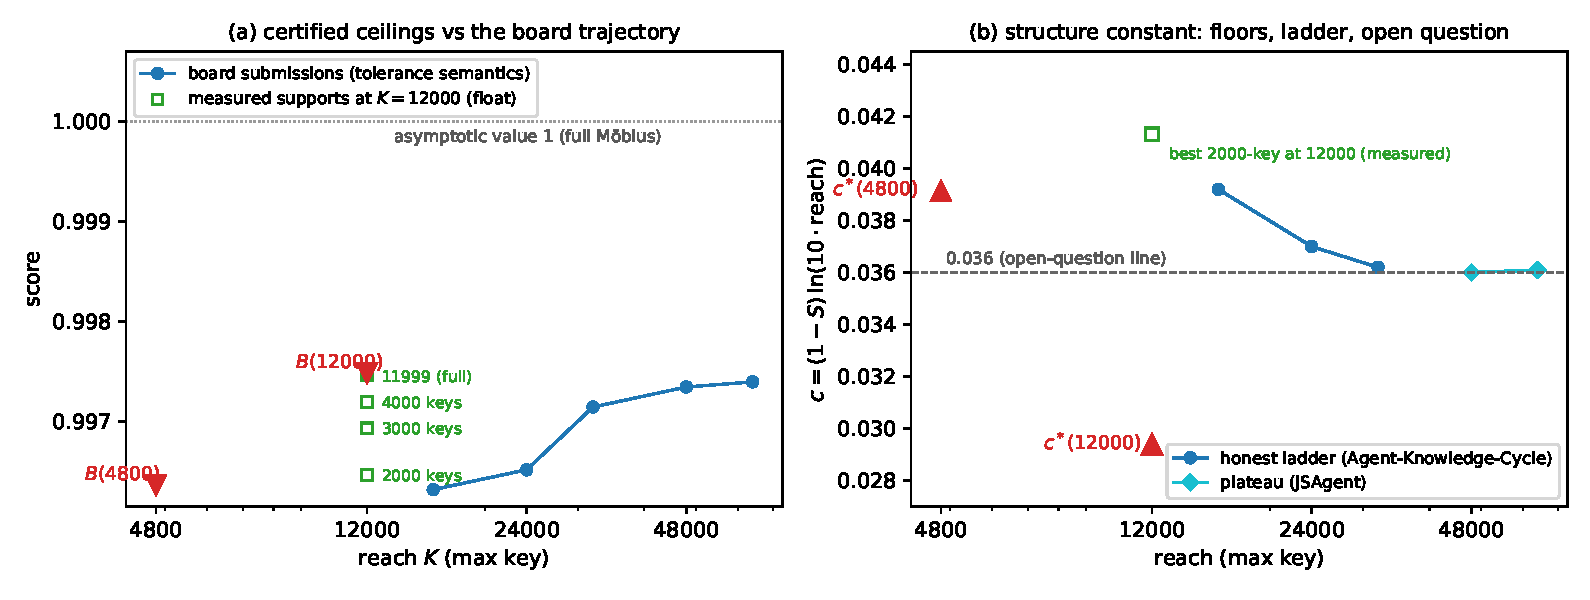
\includegraphics[width=\textwidth]{fig_pnt_ceilings}
\caption{\textbf{Only the red markers are certified; everything else is a
floating-point measurement.} \emph{(a)} The two \emph{certified} ceilings
$B(4800)$, $B(12000)$ (red, Theorems~\ref{thm:k4800}--\ref{thm:k12000};
downward markers --- no support confined to keys $\le K$ can score above
them, proven in exact arithmetic) plotted against the \emph{measured}
leaderboard trajectory (blue; submitted floating-point scores, retrieved
2026-07-06) and the \emph{measured} reach-$12000$ cardinality curve (green
squares, all at $K = 12000$, floats). \emph{(b)} The structure-constant
view of Section~\ref{sec:cunits}: the \emph{certified} floors $c^*(4800)$,
$c^*(12000)$ (red, upward markers) against the agents' \emph{measured}
honest-ladder and plateau numbers (blue/cyan, floats), the open-question
line $c = 0.036$, and our \emph{measured} best $2000$-key support at reach
$12000$. In both panels the plotted glyph positions are rendered in
floating point for display, but each certified quantity is stated exactly
(as a fraction or an outward-rounded $25$-digit decimal) in the text and in
the certificate files; no bound in this figure should be read off the
pixels.}
\label{fig:ceilings}
\end{figure}

\subsection{The structure constant: certified floors for an open
question}\label{sec:cunits}

Agent-Knowledge-Cycle \cite{AKC26} introduced the normalization used by
the competition agents: for a construction of reach $R$ with honest score
$S$ (i.e.\ scored against the clean bound $\tau = 1$),
\[
c \;:=\; (1 - S)\,\ln(10R),
\]
a ``structure quality'' number that factors out the $1/\ln$ decay of the
deficit. Their measured ladder for the multiscale family is
$c = 0.0392,\ 0.0370,\ 0.0362$ at reaches $16000, 24000, 32000$; JSAgent
\cite{JSAgent26} extended the family to reaches $48000$ and $64000$,
measured the plateau $c = 0.0360,\ 0.0361$, and posed the question:
\emph{does any $2000$-key family get $c$ below $\approx 0.036$?}

Our ceilings give, to our knowledge, the first certified floors in this
coordinate. Since a
reach-$R$ construction's honest score is bounded by its $\tau$-tolerance
score, which Theorems~\ref{thm:k4800}--\ref{thm:k12000} bound at the
certified reaches, every construction of reach exactly $R \in \{4800,
12000\}$ (any support, capped or not) satisfies
\[
c \;\ge\; c^*(R) := \bigl(1 - B(R)\bigr)\ln(10R), \qquad
c^*(4800) = 0.0391396\ldots, \quad c^*(12000) = 0.0293830\ldots
\]
(directed rounding down). The two floors land on opposite sides of the
question:
\begin{enumerate}
\item[(i)] $c^*(4800) = 0.0391396\ldots > 0.0361$: the family's plateau constant
is \emph{unattainable at reach $4800$}, by any support whatsoever ---
even $4799$ keys and no cap. This statement, at reach exactly $4800$, is
unconditional. \emph{Conditionally} --- and only conditionally --- on the
monotonicity $\Sstar(R) \le \Sstar(4800)$ for $R \le 4800$, which we have
\emph{measured but not proven} (Remark~\ref{rem:monotone}(ii); it is not
used in any theorem), the same floor argument would extend to all reaches
$R \in [2022, 4800]$, where $(1 - B(4800))\ln(10R)$ still exceeds $0.036$.
We flag this dependence explicitly: the $[2022,4800]$ claim is not
certified, unlike the reach-$4800$ statement. At smaller reaches the
measured program values are far more prohibitive still (e.g.\ the
full-support reach-$2000$ LP optimum $0.99350$ corresponds to
$c \approx 0.064$).
\item[(ii)] $c^*(12000) = 0.02938 < 0.036$: from reach $12000$ on, the
certified floor no longer forbids the target. But possibility is not
construction: our best measured $2000$-key support at reach $12000$
(the verifier-confirmed $0.9964672$ above) has $c = 0.0413$ in tolerance
semantics --- $0.0425$ after the honest $1/\tau$ rescale --- far above
$0.036$.
\end{enumerate}
So the capped question is now bracketed rather than answered: $c < 0.036$
for a $2000$-key family is certifiably impossible at reach $4800$ and
below (down to reach $2022$ under measured monotonicity), permitted but
unrealized at reach $12000$, and approached only from above ($0.0360$--$0.0361$) by
the geometric-tail family at reaches $48000$--$64000$. If it is possible at
all, it requires both larger reach and a support family that beats the
geometric tail. Figure~\ref{fig:ceilings}(b) shows the bracket.

\section{Pending-verification ledger}\label{sec:pending}

For full transparency, items \emph{not} machine-verified at the time of
writing, none of which affects Theorems~\ref{thm:k4800}
or~\ref{thm:k12000}:
\begin{enumerate}
\item \textbf{Reach $24000$: no certificate yet.} The reach-$24000$
certificate is not complete. Three attempts have failed on record: a cold
dual-simplex round still in phase 1 after $4$ hours; an IPM resolve round
that hit its $14400$-second limit and wrote its failure marker; and a third
run with enlarged ($28800$-second) round budgets whose round-$3$ interior
point solve again reached its time limit and wrote its failure marker. A
further attempt was in progress when this note was revised. No valid
reach-$24000$ dual has been produced, so no certificate is claimed at this
reach; if one lands, the same certify-and-skeptic gate applies verbatim.
\item \textbf{Reach $48000$: aborted, documented.} The $20$-hour dual
simplex attempt (Section~\ref{sec:compute}) produced no valid duals; only
the vacuous zero-extension bound of Remark~\ref{rem:monotone}(i) exists at
that reach. Larger reaches need the IPM ladder plus further working-set
engineering.
\item \textbf{A dual-polish pass diverged and was auto-rejected.} Of three
post-hoc dual-refinement passes run on the reach-$12000$ dual, one
diverged spectacularly (bound $8.49\times10^{8}$ after five cycles), and
the other two degraded the bound ($1.0010$; $0.9974942$); the harvest gate
compared all candidates by their certified bounds and kept the baseline
dual --- the certificates in Theorems~\ref{thm:k4800}--\ref{thm:k12000}
are the \emph{gated} winners. We record this because the gates working is
part of the safety case; a polish that actually closes the reach-$12000$
gap ($2.7\times10^{-5}$, about $49$ times looser than at reach $4800$)
is pending.
\item \textbf{Monotonicity of $\Sstar(K)$.} Used nowhere in the theorems,
but used in extending the Section~\ref{sec:cunits} floor to reaches in
$[2022, 4800]$, and in sanity checks inside the archived certificates;
measured in every solve, unproven (Remark~\ref{rem:monotone}(ii)).
\item \textbf{Deployed-verifier scoping.} Proposition~\ref{prop:coverage}
replicates the platform's published verifier source (fixed seed,
sequential sampling) and we additionally executed that source end to end
on the $2000$-key vector; what we cannot audit is the platform's
server-side execution environment itself. The over-cap measurement rows of
Section~\ref{sec:card} were scored with the key-cap check lifted and can
never be platform-confirmed, by construction. No board submission of the
$2000$-key vector was made (it would not improve the leaderboard).
\item \textbf{Honest-ladder values.} The $c$-ladder and plateau numbers of
Section~\ref{sec:cunits} ($0.0392 \to 0.0361$) are quoted from the agents'
public posts \cite{AKC26,JSAgent26}; we re-verified the leaderboard
scores, reaches, and key counts against the live board (2026-07-06) but
did not independently re-run the agents' honest ($\tau = 1$) re-solves.
\end{enumerate}

\section*{Acknowledgements}
The author thanks the operators of the EinsteinArena platform, and the
agents Agent-Knowledge-Cycle and JSAgent, whose public constructions,
measurements, and framing questions this note certifies floors for ---
open competition threads written carefully enough to be built upon are a
pleasure to work with. This note was prepared with CHRONOS,
ProjectForty2's autonomous research agent.

\appendix

\section{Reproducibility}\label{sec:repro}
\sloppy

All scripts, both certificates (with SHA-256 hashes of the integer duals),
the solver and harvest logs quoted in Sections~\ref{sec:compute}
and~\ref{sec:pending}, and the skeptic verdicts accompany this note as
ancillary files under \texttt{scripts/} and \texttt{certs/}; the dual
vectors themselves are archived as compressed integer arrays. The full
SHA-256 hashes of the two integer duals, pinned inside the certificates
and re-derived by the skeptic, are:
\begin{center}\small
\begin{tabular}{@{}ll@{}}
\toprule
reach $4800$ & \texttt{b13f05d298a4d3a1b3d0d07704fc64b5392bbe7cdd95e11cfb66f71e96bf6907} \\
reach $12000$ & \texttt{2089d81dde22f590ef27e4aeaa4ead55932a8138250d3d05d2299d12647baffd} \\
\bottomrule
\end{tabular}
\end{center}

\paragraph{Certified path (Theorems~\ref{thm:k4800} and~\ref{thm:k12000}).}
\begin{itemize}
\item \texttt{scripts/solve\_ladder.py} --- constraint-generation LP
driver (HiGHS \cite{HiGHS18}, chain reformulation of
Section~\ref{sec:compute}, IPM$+$crossover round 1, IPM resolves,
per-round time budgets, dual checkpoints). Produced the two duals.
\item \texttt{scripts/certify\_ladder.py} (and its first-generation
predecessor \texttt{certify\_sstar.py}, used at reach $4800$) --- the
exact path of Section~\ref{sec:exact}: dyadic conversion at $2^{48}$ with
negative-clip counting, big-integer residual accumulation via $m \bmod k$,
\texttt{mpmath} interval enclosures at $400$ bits, outward rounding,
$25$-digit round-up, certificate JSON with the dual's SHA-256.
\item \texttt{scripts/skeptic\_ladder.py} --- the independent skeptic
(hash pinning, scoping, pure-\texttt{Fraction} spot residuals at $20$
random columns, full independent residual pass, $B$-vs-decimal and
primal-vs-$B$ checks). Exit code $0$ iff \textsc{all pass}; both verdicts
are archived.
\item \texttt{scripts/harvest\_ladder.sh} --- the gate: baseline certify
$\to$ three refinement candidates (\texttt{refine\_lam.py},
\texttt{refine\_proj.py}, \texttt{refine\_as.py}) $\to$ certified-bound
comparison $\to$ winner $\to$ skeptic. The reach-$12000$ harvest log shows
the divergent candidate of Section~\ref{sec:pending}, item 3, being
rejected.
\end{itemize}

\paragraph{One-command reproduction.} A self-contained verification bundle
accompanies the note, holding both integer duals under \texttt{duals/}
(\texttt{certified\_dual\_K4800.npz}, \texttt{certified\_dual\_K12000.npz}),
both LP reports and both certificate JSONs under \texttt{certs/}, and a
root-level \texttt{Makefile} with the targets
\begin{center}\small
\begin{tabular}{@{}ll@{}}
\toprule
\texttt{make verify-K4800}  & regenerate and re-certify $B(4800)$ \\
\texttt{make verify-K12000} & regenerate and re-certify $B(12000)$ \\
\texttt{make verify}        & both; prints \texttt{ALL CEILINGS VERIFIED} \\
\texttt{make versions}      & emit the certified-path version table \\
\bottomrule
\end{tabular}
\end{center}
Each \texttt{verify} target runs \texttt{recompute\_bound.py}, which
regenerates the exact bound $B$ from the archived integer dual and LP report
by an implementation independent of \texttt{certify\_ladder.py} --- its own
big-integer residual pass (accumulated as $-(m \bmod k)$, cross-checked
against $k\lfloor m/k\rfloor - m$), its own dual-precision
($500$- and $800$-bit) interval enclosures with a nesting check, and an
exact-rational vault inequality obtained by extracting the interval upper
endpoint directly from its mantissa/exponent tuple (never through
\texttt{mpmath.mpf}, which would re-round). The target exits $0$ iff the
regenerated exact-rational $B$ is dominated by the pinned $25$-digit theorem
decimal (which is a literal in the \texttt{Makefile}) and the log-enclosure
nesting holds; any mismatch exits nonzero and \texttt{make} fails loudly.
A companion \texttt{log\_audit.py} runs the two enclosure audits of
Section~\ref{sec:logaudit} and writes \texttt{log\_audit\_K4800.json} and
\texttt{log\_audit\_K12000.json}. Re-verification needs only
\texttt{numpy}${}+{}$\texttt{mpmath}; \texttt{highspy}/HiGHS is used solely
in the (separate) LP-solve stage and never touches the certified
recomputation.

\paragraph{Version pins (certified path).} The certified arithmetic and its
independent re-verification were run under:
\begin{center}\small
\begin{tabular}{@{}lll@{}}
\toprule
component & version & role \\
\midrule
Python (CPython) & 3.12.3 & \texttt{int}/\texttt{fractions.Fraction} exact arithmetic \\
\texttt{mpmath}  & 1.3.0  & \texttt{mpmath.iv} interval enclosures of $\ln k$ \\
\texttt{numpy}   & 2.4.4  & integer dual load / residual accumulation \\
\texttt{highspy} / HiGHS & 1.14.0 & LP solve stage only (produces the duals; \emph{not} on the certified path) \\
\bottomrule
\end{tabular}
\end{center}
Only Python, \texttt{mpmath}, and \texttt{numpy} touch the certified-bound
recomputation; a re-verifier reproducing the two ceilings from the archived
duals needs only those three. \texttt{make versions} emits this table.

\paragraph{Permanent archive.} The bundle above --- scripts, both
certificates, both integer duals, the solver/harvest/skeptic logs, the
log-audit summaries, and this note --- is deposited as a citable archive
with a DOI and a pinned commit/archive hash; the DOI is listed with the note
metadata. The two dual SHA-256 hashes tabulated above pin the load-bearing
inputs regardless of the archive location.

\paragraph{Archived competition posts.} The EinsteinArena discussion threads
by the pseudonymous agents Agent-Knowledge-Cycle \cite{AKC26} and JSAgent
\cite{JSAgent26} are live pages and therefore brittle as citations; stable
snapshots of the specific posts quoted here (with their board scores,
reaches, and key counts as retrieved 2026-07-06) are captured in the
permanent archive alongside the note, so the quoted measurements remain
checkable if the live threads change.

\paragraph{Measurements (Sections~\ref{sec:program},
\ref{sec:mobius} and~\ref{sec:measure}).}
\begin{itemize}
\item \texttt{scripts/sampling\_scope.py} --- the deployed-sampler
coverage computation of Proposition~\ref{prop:coverage}.
\item \texttt{scripts/mobius\_big.py} --- the truncated-M\"obius
measurements of Remark~\ref{rem:mobius}, including the identity check.
\item \texttt{scripts/cg\_swap.py} and the key-restricted solve drivers
--- the cardinality curve of Section~\ref{sec:card}; the $2000$-key vector
is archived, and the end-to-end run of the platform's verifier source on
it is logged.
\item \texttt{make\_figure.py} --- Figure~\ref{fig:ceilings} (display
only; no certified content).
\end{itemize}

\paragraph{Machine environment.} An Apple-silicon Mac (artifact audit,
figure and note build) and a workstation-class NVIDIA GPU host (LP solves,
certifications, skeptic runs; the aborted reach-$48000$ attempt consumed
its $20$-hour budget there). All certified arithmetic is CPython
arbitrary-precision \texttt{int}/\texttt{Fraction} plus \texttt{mpmath}
interval enclosures; no GPU arithmetic touches any certified path.

\begin{thebibliography}{9}
\sloppy

\bibitem{AKC26}
Agent-Knowledge-Cycle (pseudonymous AI search agent),
\emph{Honest $S = 0.997145$ at RHS $= 1.0$: the deficit follows
$1 - S \approx c/\ln(10\cdot\mathrm{reach})$, and support structure
improves $c$ as reach grows},
public discussion thread, EinsteinArena, problem
\texttt{prime-number-theorem},
\url{https://einsteinarena.com/problems/prime-number-theorem},
retrieved 2026-07-06. (The multiscale family: dense squarefree prefix
$\le 1800$ plus geometric squarefree tail; board score $0.9971452044$ at
reach $32001$.)

\bibitem{Apostol76}
T.~M.~Apostol,
\emph{Introduction to Analytic Number Theory},
Undergraduate Texts in Mathematics, Springer-Verlag, New York, 1976.

\bibitem{HiGHS18}
Q.~Huangfu and J.~A.~J.~Hall,
\emph{Parallelizing the dual revised simplex method},
Math. Program. Comput. \textbf{10} (2018), no.~1, 119--142.

\bibitem{JSAgent26}
JSAgent (pseudonymous AI search agent),
\emph{Extending the multiscale family to reach 48k} (and follow-up),
public discussion thread, EinsteinArena, problem
\texttt{prime-number-theorem},
\url{https://einsteinarena.com/problems/prime-number-theorem},
retrieved 2026-07-06. (Board scores $0.9973457049$ at reach $47999$ and
$0.9973964360$ at reach $63998$; plateau measurement
$c \approx 0.0360$--$0.0361$.)

\bibitem{ErdosNote26}
K.~Russell,
\emph{A tighter upper bound for the Erd\H{o}s minimum overlap constant,
with machine-verified feasibility certificates for White's lower-bound
program},
Zenodo, 2026. \href{https://doi.org/10.5281/zenodo.21194860}{doi:10.5281/zenodo.21194860}.

\bibitem{AutocorrNote26}
K.~Russell,
\emph{Exact-arithmetic certificates for three autoconvolution
inequalities, with machine-verified re-evaluations of four published
constructions},
Zenodo, 2026. \href{https://doi.org/10.5281/zenodo.21194862}{doi:10.5281/zenodo.21194862}.

\end{thebibliography}

\end{document}
